\documentclass[a4paper,10pt]{article}
\usepackage[utf8x]{inputenc}
\usepackage{tikz}
\usepackage{verbatim}
\usepackage{listings}
\usepackage{float}

\setlength{\parskip}{\bigskipamount}
\setlength{\parindent}{0pt}

\usetikzlibrary{arrows}
\tikzstyle{codelabel} = [draw,rectangle]
\tikzstyle{codepart} = [minimum width=12em]
\tikzstyle{guide} = []

%opening
\title{TDT4258 Microcontrollers System Design\\Exercise 3\\[20pt]
Implementing a Multimedia Game on a Microcontroller Supported by an
Operating System}
\author{Vegard Edvardsen\\Jean Niklas L'orange\\Caroline Sæhle}

\begin{document}

\maketitle

\begin{abstract}
Handling input and output data is essential in all programs. When
developing programs for operative systems, the operative system will
provide a nice abstraction such that receiving and sending data is made
easy. When there is no operating system, one have to handle reading and
writing such data manually. This report shows how to create a C-program
which runs without an operating system on top of an STK1000 board. The
program is able to generate sound and send it to audio devices connected
through the jack socket on the board. This is done by writing to
memory-mapped I/O owned by the internal audio bitstream digital to
analog converter, which in turn handles output to the jack socket. The
I/O is performed in an interrupt routine which is consistently called by
a clock. We also explain and test out different ways of generating
sounds to the interrupt routine fast enough.

\end{abstract}

\newpage
\tableofcontents
\newpage

\section{Introduction}

The objective of this task is that the group members will get a better
understanding in how device drivers in Linux work, how to implement a
character device driver in C for the buttons and LEDs on the STK1000
board and experience on how to use device drivers in a relatively large
C program by making a game named {\em Scorched Land}. The task given to
us in the course Microcontroller System Design (TDT4258) to learn these
things was to \\
``{\em Make a driver for the use of buttons and LEDs on the STK1000. It
should be implemented as a kernel module. [\ldots] Complete the game.
Use \texttt{/dev/fb0} directly for writing to LCD screen. Use
\texttt{/dev/dsp} for producing the sound. Use your own driver for
reading the status of the buttons on STK1000. Use also your own driver
for the control of the LED diodes.  These can be used, for example, to
show how many lives a player has left or some other status information
about the game. Or you can just blink in some nice repetitive
way.}''\cite{comp}

As the specifications on how the driver exactly should work were left
unspecified, we decided to let the logic be as simple as possible:
Reading a char from the \texttt{/dev/stkboard} module gives information
about which buttons are pushed, and writing a char to the device will
set the LEDs in the configuration specified. The proper specification is
written in \ref{subsec:developing-the-driver}.

The game was developed by splitting the work in three: One to work on
integrating the device drivers with the GUI and the game, one to work on
creating and finding sounds and graphics as well as implementing code to
properly load those resouces, and one to work on the game logic. By
designing an API for image, sounds and game logic, the code became
very modular and it made testing and debugging each module on
its own an easy task.

Apart from the requirement that the game should use the driver we made,
\texttt{/dev/fb0} and \texttt{/dev/dsp}, the game logic was not
specified. The game logic was thus developed from the images in the
compendium\cite{comp} and what we already knew about the military
strategy known as scorched earth: The game designed is a turn-based game
where a soldier tries to get up to a tank, and the tank tries to block
the soldier's way by firing its gun to scorch the earth or to hit the
soldier. If there's no way for the soldier to get up to the tank or the
tank manages to hit the soldier, the tank wins. Otherwise, if the
soldier manages to get up to the tank, the soldier wins. A more detailed
specification is listed in \ref{subsec:game-logic}.


\section{Description and Methodology}

Roughly, the assignment consisted of three parts: \emph{uploading Linux}
to the microcontroller board, \emph{developing a kernel driver} for the
LEDs and buttons, and \emph{developing a game} utilizing these.

Developing the game was the most time-consuming part of the assignment.
This part consisted of several components that had to be developed. In
addition to the game logic and the user interface, the game needed
support for rendering to the screen, playing sounds, importing images,
reading hardware buttons and controlling LEDs.

\subsection{Installing Linux}

To get Linux to run on the microcontroller, a boot loader is needed in
the Flash memory as the first stage of the booting process. To upload
this boot loader, \texttt{avr32-program} was used as in the previous
assignments.

The boot loader will look for a Linux kernel on the board's memory
card. The memory card thus needs to contain a valid file system, as well
as the root file system for the OS to boot into. This was all supplied
in an image file that was ready to be written to the memory card.
Writing the image file to the card was done using \texttt{dd} on the
lab computer.

\subsection{Developing the kernel driver}
\label{subsec:developing-the-driver}
Our kernel driver follows the required steps listed in the compendium
\cite{comp}. The skeleton code was extended to perform the following
initialization steps:

\begin{itemize}
    \item Allocate a device number for a character device with
        \texttt{alloc\_chrdev\_region}.
    \item Request exclusive access to the I/O memory areas with
        \texttt{request\_region}.
    \item Set I/O registers to initialize LED output.
    \item Set I/O registers to initialize button input.
    \item Register the character device with \texttt{cdev\_add}.
\end{itemize}

Upon read requests to the device, the driver returns a single byte
representing the current data values on the button pins. Upon write
requests, the driver reads a single byte and updates the eight LED pins
accordingly.

As the PIO C port is reserved for other uses in this exercise, we needed
to use the higher bits of the PIO B port for the LEDs. However, the
mapping between bit positions in this I/O register and the physical pins
is not one-to-one. Thus, we needed to convert the physical pins to
register bits with some extra logic. The code for this is shown in
figure \ref{lst:io_mapping}.

\begin{figure}[ht]
\centering
\lstset{language=C,basicstyle=\ttfamily,numbers=left,firstnumber=28}
\begin{lstlisting}
j = i;
switch (i) {
    case 3:
    case 4:
    case 5:
    case 6: j += 2; break;
    case 7: j = 22; break;
}   
\end{lstlisting}
\caption{Logic in \texttt{driver/led.c} for I/O pin mapping. \texttt{i}
is the requested LED, \texttt{j} is the corresponding I/O pin.}
\label{lst:io_mapping}
\end{figure}


The ``protocol'' described for our device driver is thus very simple --
a single byte is the unit for both read and write operations. This
removes the need for any buffering in the driver, as well as making the
code running in kernel mode as simple as possible. The flip side is that
the application code requires more logic to handle the devices.

\subsection{Developing the game}

As mentioned in the introduction, the game consists of several components. The
game logic and the hardware interfacing (screen, sound, buttons and
LEDs) were developed in parallel. Afterwards, the user interface logic
connecting the two halves was developed. This has led to a code base
with a clean seperation of the different parts.

\subsubsection{Rendering to the screen}

Support for rendering to the screen is implemented in \texttt{screen.c}
and \texttt{screen.h}. An initialization function opens the framebuffer
device at \texttt{/dev/fb0} and uses memory mapping to allow this device
to be used as a regular C array. An in-memory array of the same size is
allocated to function as a back buffer. This is to implement double
buffering, as the image will flicker otherwise.

A custom C structure, \texttt{color\_t}, is defined, that abstracts away
the makeup of the pixels in the framebuffer array as colors with red,
green and blue components. To plot a pixel, the macro
\texttt{screen\_put} is used (see figure \ref{lst:screen_put}). This is
implemented as a macro for efficiency reasons.

\begin{figure}[ht]
\centering
\lstset{language=C,basicstyle=\ttfamily,numbers=left,firstnumber=74,breaklines=true}
\begin{lstlisting}
#define screen_put(x, y, color) (screen_buffer[(y) * SCREEN_WIDTH + (x)] = (color))
\end{lstlisting}
\caption{Pixel plotting macro in \texttt{game/screen.c}.}
\label{lst:screen_put}
\end{figure}


The function \texttt{screen\_show\_buffer} shows the back buffer on the
screen. In addition, there are several other \texttt{screen} functions
that mainly deal with drawing shapes like filled rectangles and lines.

\subsubsection{Importing image files for graphics}

For our graphics format, we chose uncompressed 24-bit \emph{Truevision
TGA} format (also known as TARGA format) for its ease of implementation
and because it is not heavily patented. Truevision TGA is a raster
graphics file format. Truevision TGA files have an 18 byte header, of
which the last 10 bytes are the image specification.

We extracted the image dimensions and format from this to find the exact
location and size of the image data, and discarded the other
information. We then rendered the raw image data directly.

% TODO: Expand

We encountered one problem: Truevision TGA format is little-endian, and
Linux on AVR32 is big-endian. Thankfully, the scope of the problem was
limited to the header of the TGA file, as the image data is given in
individual bytes. In our case, the only multiple-byte information we
needed was the image height and width, both given in two bytes. We
solved this by swapping the upper eight and lower eight bits through
bit-shifting.

\subsubsection{Playing sound effects}

We decided that a sound clip with actual music would sound better than
our rendition of ``Itsy Bitsy Spider'' from the previous exercise, and
decided upon the beginning of the Walkürenritt from Richard Wagner's
opera Der Ring des Nibelungen, as it sounds more dramatic. The source
file for the sound clip was found in the archives at Textfiles.com, and
converted to raw format using Audacity. Audacity was also used to
generate sounds where we decided not to use sound clips.

To make playback simple, we exported the sounds in raw sample format
with parameters that matched those of the \texttt{/dev/dsp} device. To
play sounds, we then only need to write the samples from the sound files
directly into \texttt{/dev/dsp}. This is implemented in \texttt{sound.c}
and \texttt{sound.h}.

\subsubsection{Reading buttons}

Reading from the hardware buttons is implemented in \texttt{button.c}
and \texttt{button.h}. Initialization is simply to open the character
device at \texttt{/dev/stkboard}, which is the driver implemented in the
previous part of this exercise. The function \texttt{btn\_read} returns
a character containing the current state of all of the eight buttons.
This is done by reading a character from \texttt{/dev/stkboard}.

The function \texttt{btn\_is\_pushed} implements further functionality to
correct unwanted button behaviour. Firstly, it reads the button state
\emph{twice}, with a sleep loop inbetween. This is to alleviate the
bouncing effects described in the first exercise.

Secondly, the function only returns true for a button \emph{once} per
button push. That is, once a button is pushed down and this is returned
from the function, the function will no longer repeat this as long as
the button is kept pushed down. This is achieved by maintaining a
\texttt{btn\_ignore} variable that masks out button pushes already
returned.

\subsubsection{Controlling LEDs}

\texttt{led.c} and \texttt{led.h} implements LED control. As with the
button support, the initialization step is to open the
\texttt{/dev/stkboard} device.

\subsubsection{Implementing the game logic}
\label{subsec:game-logic}
The game logic itself is implemented in \texttt{scorched\_land.c} and the
API created with documentation is implemented in
\texttt{scorched\_land.h}. By separating game logic from the
STK1000-specific implementation, one can implement the game on another
platform without the need to reimplement the game logic. This made it
possible to make a simple terminal version of the game with colours for
linux to debug the game logic, without the need of a GUI on the STK1000
board. 

As there were no specifications on how the game logic should work, we
decided to make a game logic specification before implementing the game.
We ended up with the following specifications on how the game should
work:
\begin{itemize}
    \item The game is grid-based where the soldier uses 1x1 space, and
            begins initially in the lower left corner.
    \item The tank uses 2x2 space and is placed in the top right corner.
    \item The soldier is able to move in the directions north, west, up
            and down if and only if the tile the soldier wants to move
            to is within the grid size and the tile is not scorched land.
    \item The tank is stationary, and can shoot a gun which will scorch
            the land. The player gives an angle and a strenght on the
            shot, and the game will calculate where the shot ends up at.
    \item The soldier will win if he gets to a tile which is
            occupied by the tank.
    \item The tank will win if he hits the soldier, or if the hit makes
            it impossible to reach the tank for the soldier.
\end{itemize}

We decided to omit details such as grid size and whether the game is
turn based or real-time in the specifications, and instead make it
possible to change these choices at compile-time.

After we had decided on specification details, we implemented the
API in the \texttt{scorched\_land.h} file, with explanation on what
parameters each function takes, what the function does, and what you can
expect from the return parameter. When we finished the API, we started
implementing the game in the \texttt{scorched\_land.c} file.

The game is initialized by running the \texttt{game\_init} function.
This will reset all variables related to the game in case these values
have not been previously initialized, or if one has already played a
game and wants to start over. To let the tank shoot a bullet, one calls
the function \texttt{game\_shoot\_bullet} with two integers: One
denoting the direction in degrees the bullet is supposed to go, the
second denoting how much power to use - which determines how far the
bullet goes.

\begin{figure}[ht]
\centering
\lstset{language=C,basicstyle=\ttfamily,numbers=left,firstnumber=42}
\begin{lstlisting}
    double radians = ( direction ) * ( M_PI / 180 ),
           x_multiplier = cos ( radians ),
           y_multiplier = sin ( radians ),
           scaled_strength = strength *  GAME_STRENGTH_SCALE;

    int    x = (int) ( x_multiplier * scaled_strength ),
           y = (int) ( y_multiplier * scaled_strength );
    /* Flip the x-position. */
    x = GAME_WIDTH - 1 - x;
\end{lstlisting}
\caption{Logic in \texttt{game/scorched\_land.c} to calculate which tile to hit.}
\label{lst:pos-code}
\end{figure}


Calculating where the bullet lands is done by the code snippet shown in
figure \ref{lst:pos-code}. We first convert the degrees to radians. We
then find out how far on the x- and y-axis the shot goes by calculating
the sine and cosine of the radians we just calculated. This is in turn
multiplied by a previously calculated factor
\texttt{GAME\_STRENGTH\_SCALE} and the strength given as parameter, and
then rounded down to an integer. Finally, we flip the x-position to
let the shot go from the correct corner.

\texttt{GAME\_STRENGTH\_SCALE} is calculated by taking the longest total
distance a shot can go divided by \texttt{GAME\_MAX\_STRENGTH}, the
maximal power one can shoot with.  The longest total distance a shot can
go is $\sqrt{W^2 + H^2}$ where $W = $\texttt{GAME\_WIDTH} and $H =$
\texttt{GAME\_HEIGHT} length.  By multiplying by this factor, we ensure
that the tank is able to hit any tile on the game regardless of maximal
strength and game dimensions. 

\begin{figure}[ht]
\centering
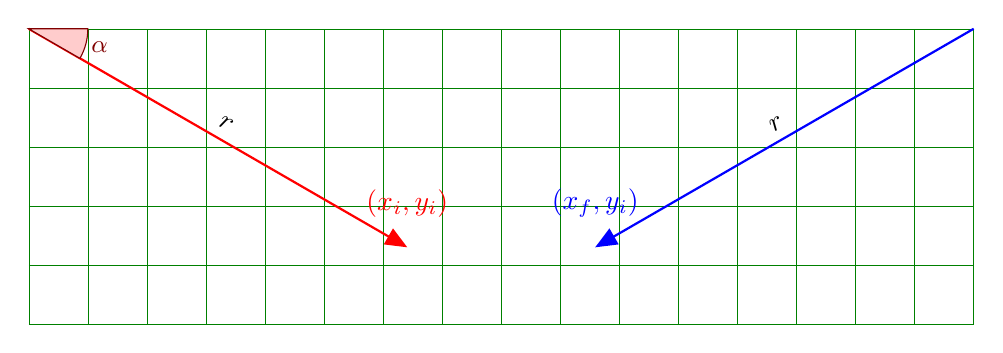
\begin{tikzpicture}

\draw[step=0.75cm,color=green!50!black,very thin] (0,-3.75) grid (12,0);

\draw[triangle 45-,color=red, thick]
    (330:5.55) node[above=7pt] {$(x_i,y_i)$} -- 
    (0,0) node[midway,sloped,above,color=black]{$r$};

\draw[fill=red!20,draw=red!50!black] 
    (0,0) -- (0.75, 0) arc (0:-30:0.75) -- cycle; 

\draw[color=red!50!black]
    (0,0) node[right=0.9cm, below=0.045cm]{{\small $\alpha$}};

\draw[triangle 45-,color=blue, thick] 
    (12,0) ++(210:5.55cm) node[above=7pt]{$(x_f,y_i)$}
               -- (12,0) node[midway,sloped,above,color=black]{$r$};

\end{tikzpicture}
\caption{Calculating the landing position of a gun shot. The red arrow
represents the calculated values before flipping the x-position, and the
blue arrow represents the calculated values afterwards.}
\label{fig:pos-calc}
\end{figure}



The function \texttt{game\_move\_player} will move the soldier with the
specified direction you want the soldier to go to, if possible. The
function will check whether the position is ok to move to, and if so,
will move the soldier from its current position to its next. Finally,
the functions returns a reasonable response which gives the GUI
possibility to properly give error messages if wanted.

After the initial implementation, a terminal version of the game was
created to test the functionality and check that all worked as intended.
The terminal version can be compiled and run by running the command 
\verb|make test && test/sc_land| in the \texttt{game} folder, or
through \verb|make && ./sc_land| in the \texttt{game/test} folder.

\begin{figure}[ht]
\centering
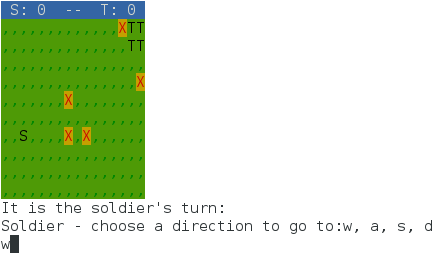
\includegraphics[scale=0.6]{screenshots/terminal003.png}
\caption{The terminal implementation (\texttt{sc\_land}) of the game.}
\label{fig:terminal-screenshot-0}
\end{figure}


By implementing a terminal version, we could test the implementation
much faster and debug with the "GNU Debugger" available, which give a
much better debug support than the STK1000 board does. From the
implementaion, we found and solved bugs in regards to correctly placing
scorched land from a bullet shot. We also found out that we forgot to
flip the x-axis, and implemented the code needed to flip it.


\section{Results and tests}

Testing of the sound production was performed in successive stages, as
we refined the code. Tests consisted of uploading the code and listening
to the result, using the headphones. One of the group members is a hobby
musician with relative pitch and performed the more advanced listening
tests.

\subsection{Prerequisites for testing:}
\begin{itemize}
\item Code compiles and is uploaded to microcontroller.
\item Headphones in jack socket.
\item For pitch-specific tests, person easily able to distinguish between frequencies (relative pitch).
\item Trusted sound generator for pitch comparison to absolute frequencies (we used Audacity 1.3 Beta).
\item Standard pitch is Concert A, 440Hz.
\end{itemize}

\subsection{Terms and expressions used in tables}
\begin{itemize}
\item ``Reasonably clear note'' denotes a clear tone with only light
noise on top. Some light noise is to be expected due to our hardware,
and is ignored for testing purposes, as there is no way to change this.
\item ``Noise'' refers to significant noise, such as low buzzes, high
beeps, and other noise that goes well beyond the expected light noise.
\item ``Consistent'' means that the pitch of the output and the
pitch of the trusted sample sound are indistinguishable.
\end{itemize}

Our first implementation used a random number generator as input.
Test 1:
\begin{center}
\begin{tabular}{|p{3.6cm}|p{3.6cm}|p{3.6cm}|}
\hline
{\sc Test} & {\sc Expected outcome} & {\sc Observed outcome}\\ \hline
Do we have sound? & Yes. & Yes.\\ \hline
Do we have noise? & Yes, given our random input. & Yes. \\ \hline
Do we have a reasonably clear note? & No. & No. We did not have a clear note at all, as expected.\\ \hline
\end{tabular}
\end{center}
After this, we tried implementing a sine wave directly with a frequency
of 440hz.
Test 2:
\begin{center}
\begin{tabular}{|p{3.6cm}|p{3.6cm}|p{3.6cm}|}
\hline
{\sc Test} & {\sc Expected outcome} & {\sc Observed outcome}\\ \hline
Do we have sound? & Yes. & Yes. \\ \hline
Do we have a reasonably clear note? & Yes. & No. {\em Test failed.} \\ \hline
Do we have noise beyond this? & No. & No. \\ \hline
Do we have a pitch consistent with A440? & Yes. & No. {\em Test failed.} \\
\hline
\end{tabular}
\end{center}

As a result of this test, we moved the sine calculation out of the
interrupt handler, and into a sine lookup table.
Test 3:
\begin{center}
\begin{tabular}{|p{3.6cm}|p{3.6cm}|p{3.6cm}|}
\hline
{\sc Test} & {\sc Expected outcome} & {\sc Observed outcome}\\ \hline
Do we have sound? & Yes. & Yes. \\ \hline
Do we have a reasonably clear note? & Yes. & Yes. \\ \hline
Do we have noise beyond this? & No. & No. \\ \hline
Do we have a pitch consistent with A440? & Yes. & No. {\em Test failed.} \\
\hline
\end{tabular}
\end{center}

However, due to ending up with the wrong tone we suspected that our interrupt handler still took up too much
time, and that samples were not delivered sufficiently fast enough.

We tested this by successively dividing the rate by 2, 4, and 8. Seeing as this was the only difference in our code, we only compared the resulting pitch with 440Hz.
Rate divisor  |	Consistent with A440?
2 				No
4				No
8				Yes

We concluded that our interrupt handler took too much time by a factor
of approximately eight. As a result of this, we realised that our method
was still too slow, and decided to change our lookup table entirely,
changing to a sound buffer. The sound buffer contains all the
pre-calculated samples. //TODO:(REF to earlier text!) After this change,
we decided to test it again.

Test 4:
\begin{center}
\begin{tabular}{|p{3.6cm}|p{3.6cm}|p{3.6cm}|}
\hline
{\sc Test} & {\sc Expected outcome} & {\sc Observed outcome}\\ \hline
Do we have sound? & Yes. & Yes. \\ \hline
Do we have a reasonably clear note? & Yes. & Yes. \\ \hline
Do we have noise beyond this? & No. & No. \\ \hline
Do we have a pitch consistent with A440? & Yes. & Yes. \\ \hline
\end{tabular}
\end{center}

We were now able to produce a note given a certain frequency. We
continued by implementing octaves. Octaves are half or double the
frequency, and are perceived by the human ear to be alike. This makes
them easy to test for. We used the buttons to control this. Pressing the
left button (button 3) would make the function double the frequency (up
one octave), and pressing the right button (button 1) would halve the
frequency (going down one octave).

Test 5:
\begin{center}
\begin{tabular}{|p{3.6cm}|p{3.6cm}|p{3.6cm}|}
\hline
{\sc Test} & {\sc Expected outcome} & {\sc Observed outcome}\\ \hline
Do we have sound? & Yes. & Yes. \\ \hline
Do we have a reasonably clear note? & Yes. & Yes. \\ \hline
Do we have noise beyond this? & No. & No. \\ \hline
Do the buttons react to pressing? & Yes. & Yes. \\ \hline
Does the left button shift the pitch up? & Yes. & Yes. \\ \hline
Does the right button shift the pitch down? & Yes. & Yes. \\ \hline
At button press, is the pitch change up or down consistent to octaves? &
Yes. & Yes. \\ \hline
\end{tabular}
\end{center}

We then implemented the chromatic scale using the standard semitone
frequency ratio [Twelfth root of two] and using 440Hz as a reference
point, binding the first eight semitones starting from C4 to the eight
buttons, in theory giving us a range of C4 to G4. If correct, the pitch
would increase by a semitone for each higher button pressed, and the
buttons for C (1), E (5), and G(8) would give us a sequence called a
major triad (in this case a C major triad). This sequence is very easily identifiable even to
non-musicians, as it is found in most popular music.

Test 6:
\begin{center}
\begin{tabular}{|p{3.6cm}|p{3.6cm}|p{3.6cm}|}
\hline
{\sc Test} & {\sc Expected outcome} & {\sc Observed outcome}\\ \hline
Do we have sound? & Yes. & Yes.\\ \hline
Do we have a reasonably clear note? & Yes. & Yes. \\ \hline
Do we have noise beyond this? & No. & No. \\ \hline
Do the buttons react to pressing? & Yes. & Yes.\\ \hline
Does a successive pressing of buttons 1-8 play the correct notes? & Yes. & No.\\ \hline
Does the C major triad play correctly? & Yes. & No.\\ \hline
\end{tabular}
\end{center}

At first, we were puzzled at this, and started checking whether we had made an error in calculating the right frequency. However, double-checking the code showed that we had indeed used the
correct formula for the pitch as far as we could see, and we
decided to test it again by implementing note sequence arrays
(melodies), instead of directly binding the tones to the buttons. For
melodies, we chose simple, well-known children's songs so that the
entire group would easily be able to identify any errors.

Test 7:
\begin{center}
\begin{tabular}{|p{3.6cm}|p{3.6cm}|p{3.6cm}|}
\hline
{\sc Test} & {\sc Expected outcome} & {\sc Observed outcome}\\ \hline
Do we have sound? & Yes. & Yes.\\ \hline
Do we have a reasonably clear note? & Yes. & Yes. \\ \hline
Do we have noise beyond this? & No. & No. \\ \hline
Do the buttons react to pressing? & Yes. & Yes.\\ \hline
Do the melodies perform in tune as coded with pitch references? & Yes. &
Yes. \\ \hline
\end{tabular}
\end{center}

Our test established that the fault must have been somewhere else, and we
continued implementing melodies and note sequences as planned. We
decided that we also needed to find a way to make silences, as our
melodies needed short pauses between certain notes.

\begin{center}
\begin{tabular}{|p{5cm}|p{5cm}|}
\hline
{\sc Attempted solution} & {\sc Result} \\ \hline
Very low frequency.	& Faint crackling noise, buzzing and beeping.  \\ \hline
Very high frequency. & Loud buzz.  \\ \hline
Gradually lowering the amplitude. & Faint crackling noise, buzzing and beeping. Gradual fade-out of tone. \\ \hline
\end{tabular}
\end{center}

We have not been able to eliminate this noise, but eventually ended up
choosing to use a very low frequency, as this noise was the least
annoying. This was implemented by using a buffer with one element of
value 0. Having decided this, we implemented ``Itsy Bitsy Spider'' with
pauses as our introduction melody, along with a few other sequences for
a win, firing, and a hit.

Test 8:
\begin{center}
\begin{tabular}{|p{3.6cm}|p{3.6cm}|p{3.6cm}|}
\hline
{\sc Test} & {\sc Expected outcome} & {\sc Observed outcome}\\ \hline
Do we have sound? & Yes. & Yes. \\ \hline
Do we have a reasonably clear note? & Yes. & Yes. \\ \hline
Do we have noise beyond this? & No. & Yes, we did, during the recently implemented silences. \\ \hline
Reasonably clear note? & Yes. & Yes. \\ \hline
Do the buttons react to pressing? & Yes. & Yes. \\ \hline
Do the melodies perform in tune as coded with pitch references? & Yes. &
Yes. \\ \hline
\end{tabular}
\end{center}

\section{Evaluation of the assignment}

This was a suitable challenge for computer science students who have not
worked with processors at an assembly level before. We needed to use
``trial and error'' methods to solve the assignment, and we consider
this a good way to learn about the architecture of a microprocessor and
the programs used in development of microprocessor software.

It was easy to know where to start thanks to the good assignment
description, and we could try out a small program and then develop that
small program into a solution to the assignment without having to
redesign the whole thing. It was also easy to test whether the assembly
code you had programmed worked as intended through the usage of {\em
STK1000 development board} and the {\em GNU Debugger}.

The assignment provided practical and useful experience that feels
relevant considering the study line and future courses. It seems likely
that we will need what we learnt during the execution of the assigment
sometime in the future.

\begin{comment}
Writing such a thorough report is a relatively new activity for the
members of our group, so we were a little uncertain as to how thorough
the report was supposed to be. An example report for some assignment in
the same field would useful, so that we would know whether we're doing
it right or not. The approximate expected report length could also have
been specified.
\end{comment}

\section{Conclusion}

We completed the assignment with the recommended approach given in the
compendium. By doing this, we learnt how programming a microcontroller
in C is done, as well as doing interrupt handling and memory-based I/O
on an AVR32. In addition, we decided to use a sine wave to generate
sound, which required more work than any of the other waves we could
have used instead. By doing this, we learnt how to bypass computation
heavy sound generation by either pregenerating a single period of a tone
just before it is needed, or by pregenerating all tones used at the
start of the program. 

As we were not completely satisfied with the noise generated during
``silence'', we tested out many different ways to try to solve the issue.
However, though we were unable to solve the problem, we found a plausible reason
for the noise, as well as a possible solution. Unfortunately, we did not
have time enough to try out this solution, as it required a major
refactoring.

\begin{thebibliography}{9}

\bibitem{comp}
    NTNU,
    \emph{Lab Assignments in TDT4258 Microcontroller System Design},
    Computer Architecture and Design Group,
    Department of Computer and Information Science,
    Norwegian University of Science and Technology,
    2011.

\bibitem{tga}
    Wikipedia,
    \emph{Truevision TGA},
    http://en.wikipedia.org/wiki/Truevision\_TGA,
    accessed 2012-05-04.

\end{thebibliography}


\end{document}
